\chapter{Модель и алгоритмы для решения задачи сегментации и классификации крюков}

\section{Модификация модели представления результатов сегментации страницы с крюками и знамёнами}

Модель представления результатов сегментации и классификации букв выполнена с использованием технологии HOCR, который является HTML-подобным 
форматом, разработанным для хранения информации о распознанных текстах, их координатах и структурных элементах. 
Этот формат позволяет легко интегрировать результаты сегментации в веб-приложения и обеспечивает гибкость в 
обработке текстов\cite{MMemon}.


Однако на данный момент нейросетевая модель для распознавания крюков не готова к полноценному использованию. 
Результаты ее работы недостаточно точны, а производительность оставляет желать лучшего. 

% \begin{figure}[H]
%   \begin{center}
%     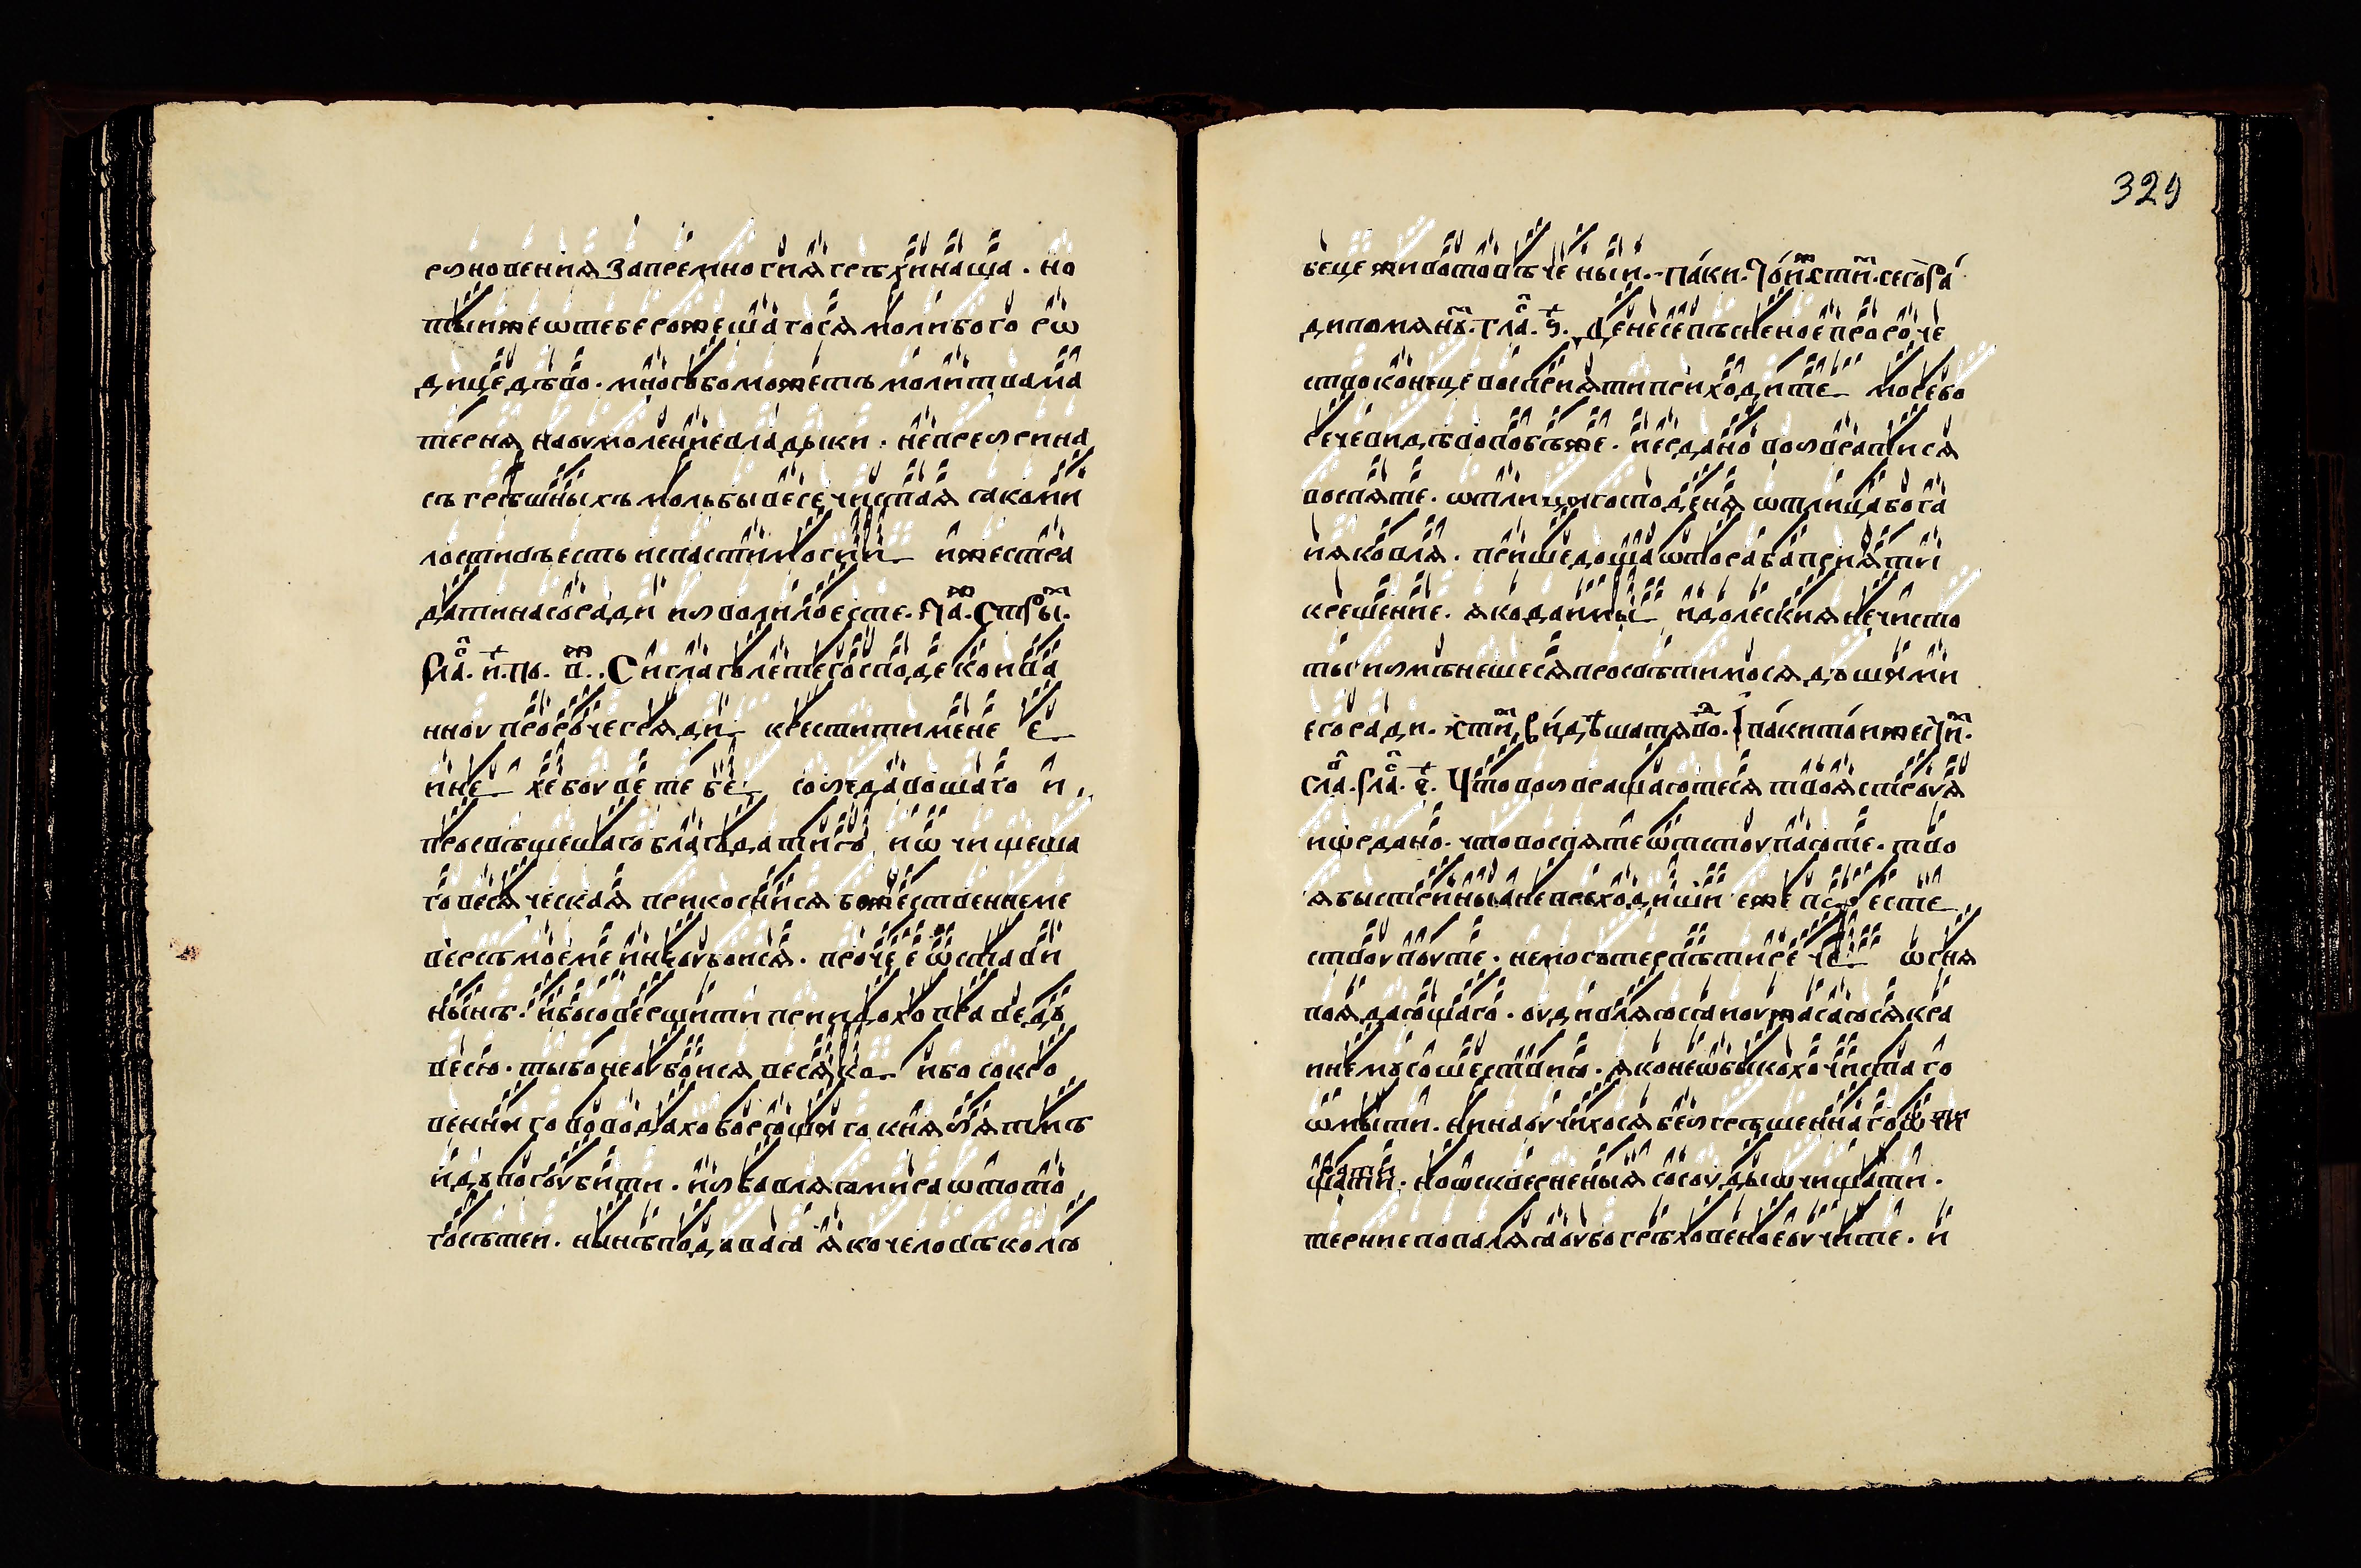
\includegraphics[width=.9\columnwidth]{./img/badNeuro.jpg}%
%   \end{center}
%   \caption{Пример обработки страницы нейросетью на текущий момент.}%
%   \label{pic:badNeuro}%
% \end{figure}


Основной задачей этой работы является участие в разработке портала, поэтому полноценное представление крюков в формате HOCR 
наравне с буквами – это задача не ближайшей перспективы.

Вместо этого, на данном этапе разработки необходимо сфокусироваться на модели, которая сможет ответить на вопрос: 
"Имеются ли крюки и знамена на данной странице рукописи?" Это позволит определить целесообразность запуска более 
сложной нейросетевой модели, процесс которой долгий и в текущем состоянии приводит к неточным результатам.

Для соответствия требованию определения наличия крюков на странице, модель должна содержать представление крюков 
для их линейного поиска. Результаты этого поиска должны включать информацию о количестве крюков и их расположении 
на странице.

Количество крюков является ключевым параметром, на основе которого будет приниматься решение о необходимости 
запуска нейросети. Расположение крюков служит вспомогательным атрибутом, необходимым для отслеживания и 
диагностики ошибок в случае неправильной сегментации или классификации. Точное указание местоположения крюков 
позволит эффективно выявлять и корректировать возможные недостатки в работе модели, обеспечивая более 
надежную и точную обработку данных.

Тогда модель классификации и сегментации крюков и знамен имеет вид:

\begin{figure}[H]
  \begin{center}
    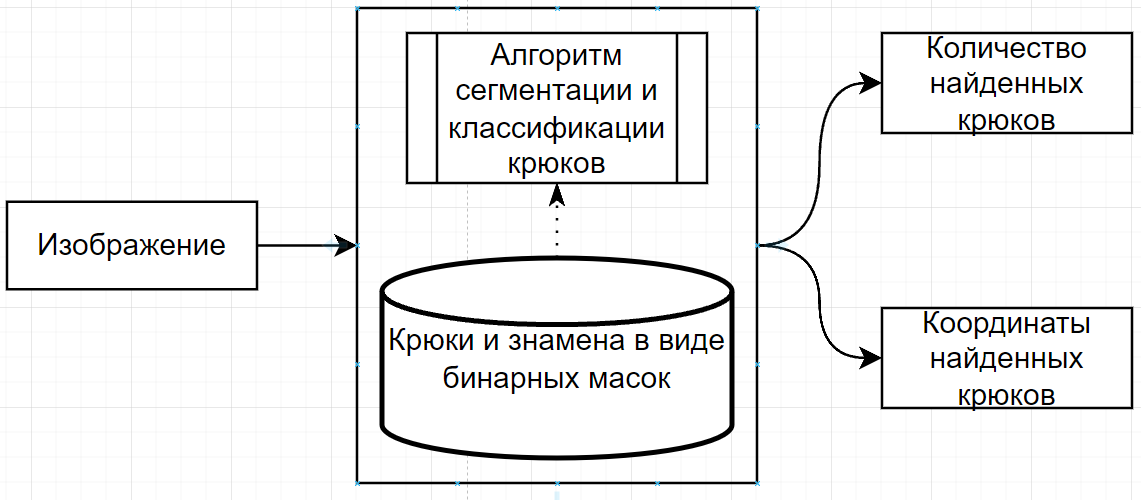
\includegraphics[width=.5\columnwidth]{./img/sysModel.png}%
  \end{center}
  \caption{Модель классификации и сегментации крюков и знамен.}%
  \label{pic:algo}%
\end{figure}



\section{Алгоритм генерации редактируемой цифровой копии страницы с крюками и знамёнами}

По описанным причинам из прошлого пункта, основная цель алгоритма — классификация крюков для определения 
необходимости запуска нейросетевой модели.

В качестве способа поиска крюков по маскам, выбран алгоритм сопоставления с шаблоном.

\begin{figure}[H]
  \begin{center}
    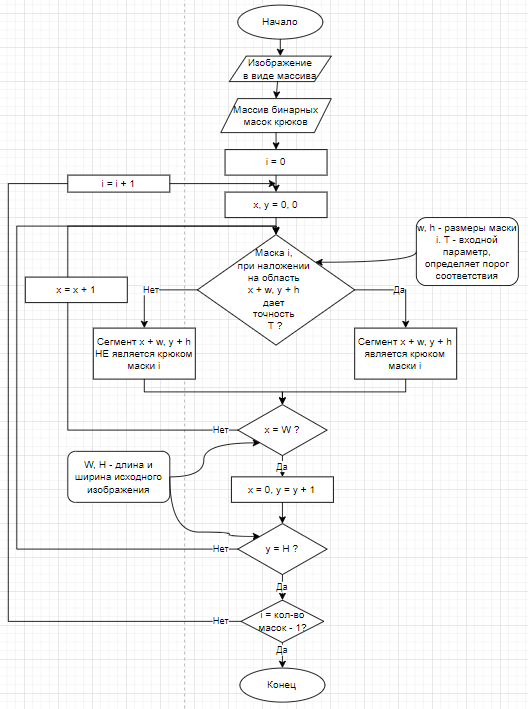
\includegraphics[width=.8\columnwidth]{./img/algo.png}%
  \end{center}
  \caption{Диаграмма алгоритма сопоставления с шаблоном.}%
  \label{pic:algo}%
\end{figure}

Метод сопоставления с шаблоном представляет собой процесс поиска и идентификации участков изображения, которые 
соответствуют заранее определённым шаблонам. В случае нашего исследования, шаблонами являются бинарные маски 
крюков и знамен. Метод включает наложение шаблона на изображение и оценку степени совпадения, чтобы определить 
участки наиболее подходящих под шаблон.

В качестве метрики степени совпадения между шаблоном и изображением используется нормализованная сумма произведений:
\begin{center}
  $R(x, y) = \frac{1}{N} \sum_{i=0}^{w-1} \sum_{j=0}^{h-1} T(i, j) \cdot I(x + i, y + j)$
\end{center}
Где:
\begin{itemize}
  \item \( R(x, y) \) — степень совпадения на координатах \( (x, y) \).
  \item \( T(i, j) \) — значение пикселя шаблона в координатах \( (i, j) \).
  \item \( I(x + i, y + j) \) — значение пикселя изображения в координатах \( (x + i, y + j) \).
  \item \( w \) и \( h \) — ширина и высота шаблона соответственно.
  \item \( N \) — общее количество пикселей в шаблоне (\( N = w \cdot h \)).
\end{itemize}

Параметр \( R(x, y) \) будет оцениваться пороговом значением \( T \), которое будет определять принадлежность сегмента
изображения к крюку или знамени

Нормализованная сумма произведений была выбрана как метод оценки схожести шаблона и изображения, из-за своей быстроты, легкости в реализации, а также
инвариантности к яркости\cite{MGonsales}.

\section{Выводы}

В результате разработки модели и алгоритмов была представлена модель, эффективно решающая задачу классификации 
крюков и знамен для определения необходимости использования нейросетевой модели. Использование подхода 
бинарных масок и шаблонного сопоставления позволяет достичь высокого быстродействия, что важно для 
оперативного принятия решений. Модель является легковесной и дообучаемой, что обеспечивает 
её адаптируемость при расширении выборки данных.

%%% Local Variables:
%%% TeX-engine: xetex
%%% eval: (setq-local TeX-master (concat "../" (seq-find (-cut string-match ".*-3-pz\.tex$" <>) (directory-files ".."))))
%%% End:
